\documentclass[]{book}
\usepackage{lmodern}
\usepackage{amssymb,amsmath}
\usepackage{ifxetex,ifluatex}
\usepackage{fixltx2e} % provides \textsubscript
\ifnum 0\ifxetex 1\fi\ifluatex 1\fi=0 % if pdftex
  \usepackage[T1]{fontenc}
  \usepackage[utf8]{inputenc}
\else % if luatex or xelatex
  \ifxetex
    \usepackage{mathspec}
  \else
    \usepackage{fontspec}
  \fi
  \defaultfontfeatures{Ligatures=TeX,Scale=MatchLowercase}
\fi
% use upquote if available, for straight quotes in verbatim environments
\IfFileExists{upquote.sty}{\usepackage{upquote}}{}
% use microtype if available
\IfFileExists{microtype.sty}{%
\usepackage{microtype}
\UseMicrotypeSet[protrusion]{basicmath} % disable protrusion for tt fonts
}{}
\usepackage[margin=1in]{geometry}
\usepackage{hyperref}
\hypersetup{unicode=true,
            pdftitle={Methods Comparison},
            pdfborder={0 0 0},
            breaklinks=true}
\urlstyle{same}  % don't use monospace font for urls
\usepackage{natbib}
\bibliographystyle{apalike}
\usepackage{color}
\usepackage{fancyvrb}
\newcommand{\VerbBar}{|}
\newcommand{\VERB}{\Verb[commandchars=\\\{\}]}
\DefineVerbatimEnvironment{Highlighting}{Verbatim}{commandchars=\\\{\}}
% Add ',fontsize=\small' for more characters per line
\usepackage{framed}
\definecolor{shadecolor}{RGB}{248,248,248}
\newenvironment{Shaded}{\begin{snugshade}}{\end{snugshade}}
\newcommand{\KeywordTok}[1]{\textcolor[rgb]{0.13,0.29,0.53}{\textbf{#1}}}
\newcommand{\DataTypeTok}[1]{\textcolor[rgb]{0.13,0.29,0.53}{#1}}
\newcommand{\DecValTok}[1]{\textcolor[rgb]{0.00,0.00,0.81}{#1}}
\newcommand{\BaseNTok}[1]{\textcolor[rgb]{0.00,0.00,0.81}{#1}}
\newcommand{\FloatTok}[1]{\textcolor[rgb]{0.00,0.00,0.81}{#1}}
\newcommand{\ConstantTok}[1]{\textcolor[rgb]{0.00,0.00,0.00}{#1}}
\newcommand{\CharTok}[1]{\textcolor[rgb]{0.31,0.60,0.02}{#1}}
\newcommand{\SpecialCharTok}[1]{\textcolor[rgb]{0.00,0.00,0.00}{#1}}
\newcommand{\StringTok}[1]{\textcolor[rgb]{0.31,0.60,0.02}{#1}}
\newcommand{\VerbatimStringTok}[1]{\textcolor[rgb]{0.31,0.60,0.02}{#1}}
\newcommand{\SpecialStringTok}[1]{\textcolor[rgb]{0.31,0.60,0.02}{#1}}
\newcommand{\ImportTok}[1]{#1}
\newcommand{\CommentTok}[1]{\textcolor[rgb]{0.56,0.35,0.01}{\textit{#1}}}
\newcommand{\DocumentationTok}[1]{\textcolor[rgb]{0.56,0.35,0.01}{\textbf{\textit{#1}}}}
\newcommand{\AnnotationTok}[1]{\textcolor[rgb]{0.56,0.35,0.01}{\textbf{\textit{#1}}}}
\newcommand{\CommentVarTok}[1]{\textcolor[rgb]{0.56,0.35,0.01}{\textbf{\textit{#1}}}}
\newcommand{\OtherTok}[1]{\textcolor[rgb]{0.56,0.35,0.01}{#1}}
\newcommand{\FunctionTok}[1]{\textcolor[rgb]{0.00,0.00,0.00}{#1}}
\newcommand{\VariableTok}[1]{\textcolor[rgb]{0.00,0.00,0.00}{#1}}
\newcommand{\ControlFlowTok}[1]{\textcolor[rgb]{0.13,0.29,0.53}{\textbf{#1}}}
\newcommand{\OperatorTok}[1]{\textcolor[rgb]{0.81,0.36,0.00}{\textbf{#1}}}
\newcommand{\BuiltInTok}[1]{#1}
\newcommand{\ExtensionTok}[1]{#1}
\newcommand{\PreprocessorTok}[1]{\textcolor[rgb]{0.56,0.35,0.01}{\textit{#1}}}
\newcommand{\AttributeTok}[1]{\textcolor[rgb]{0.77,0.63,0.00}{#1}}
\newcommand{\RegionMarkerTok}[1]{#1}
\newcommand{\InformationTok}[1]{\textcolor[rgb]{0.56,0.35,0.01}{\textbf{\textit{#1}}}}
\newcommand{\WarningTok}[1]{\textcolor[rgb]{0.56,0.35,0.01}{\textbf{\textit{#1}}}}
\newcommand{\AlertTok}[1]{\textcolor[rgb]{0.94,0.16,0.16}{#1}}
\newcommand{\ErrorTok}[1]{\textcolor[rgb]{0.64,0.00,0.00}{\textbf{#1}}}
\newcommand{\NormalTok}[1]{#1}
\usepackage{longtable,booktabs}
\usepackage{graphicx,grffile}
\makeatletter
\def\maxwidth{\ifdim\Gin@nat@width>\linewidth\linewidth\else\Gin@nat@width\fi}
\def\maxheight{\ifdim\Gin@nat@height>\textheight\textheight\else\Gin@nat@height\fi}
\makeatother
% Scale images if necessary, so that they will not overflow the page
% margins by default, and it is still possible to overwrite the defaults
% using explicit options in \includegraphics[width, height, ...]{}
\setkeys{Gin}{width=\maxwidth,height=\maxheight,keepaspectratio}
\IfFileExists{parskip.sty}{%
\usepackage{parskip}
}{% else
\setlength{\parindent}{0pt}
\setlength{\parskip}{6pt plus 2pt minus 1pt}
}
\setlength{\emergencystretch}{3em}  % prevent overfull lines
\providecommand{\tightlist}{%
  \setlength{\itemsep}{0pt}\setlength{\parskip}{0pt}}
\setcounter{secnumdepth}{5}
% Redefines (sub)paragraphs to behave more like sections
\ifx\paragraph\undefined\else
\let\oldparagraph\paragraph
\renewcommand{\paragraph}[1]{\oldparagraph{#1}\mbox{}}
\fi
\ifx\subparagraph\undefined\else
\let\oldsubparagraph\subparagraph
\renewcommand{\subparagraph}[1]{\oldsubparagraph{#1}\mbox{}}
\fi

%%% Use protect on footnotes to avoid problems with footnotes in titles
\let\rmarkdownfootnote\footnote%
\def\footnote{\protect\rmarkdownfootnote}

%%% Change title format to be more compact
\usepackage{titling}

% Create subtitle command for use in maketitle
\newcommand{\subtitle}[1]{
  \posttitle{
    \begin{center}\large#1\end{center}
    }
}

\setlength{\droptitle}{-2em}

  \title{Methods Comparison}
    \pretitle{\vspace{\droptitle}\centering\huge}
  \posttitle{\par}
    \author{Malu Calle Rosingana\\
Coding: Yiwen Wang}
    \preauthor{\centering\large\emph}
  \postauthor{\par}
      \predate{\centering\large\emph}
  \postdate{\par}
    \date{2019-02-26}

\usepackage{booktabs}
\usepackage{amsthm}
\makeatletter
\def\thm@space@setup{%
  \thm@preskip=8pt plus 2pt minus 4pt
  \thm@postskip=\thm@preskip
}
\makeatother


\usepackage{fancyhdr}
\usepackage{hyperref}
\usepackage{lipsum}
\setlength{\headheight}{28pt}
\setlength{\footskip}{25pt}
\pagestyle{fancy}
\renewcommand{\headrulewidth}{0.5pt}
\renewcommand{\footrulewidth}{0.5pt}
\lhead{
\includegraphics[width=10cm,height=1.2cm]{logo.jpg}}
\cfoot{\scriptsize Universitat de Vic | Univerisitat Central de Catalunya}
\rfoot{\scriptsize \thepage}
\fancyhead[R]{\slshape\leftmark}
\fancypagestyle{plain}{\pagestyle{fancy}}

\usepackage{fontspec}
\setmainfont{Times New Roman}

\begin{document}
\maketitle

{
\setcounter{tocdepth}{3}
\tableofcontents
}
\chapter{Introduction}\label{introduction}

This vignette provides a comparison of the 12 variables selected by the
3 methods: coda\_logistic\_lasso, clr+logistic\_lasso, selbal.

First, let us install and load the packages.

\section{Packages installation and
loading}\label{packages-installation-and-loading}

\begin{Shaded}
\begin{Highlighting}[]
\CommentTok{#cran.packages = c('knitr','MASS','VennDiagram','gplots','glmnet')}
\CommentTok{#install.packages(cran.packages)}
\CommentTok{#devtools::install_github(repo = "UVic-omics/selbal")}

\KeywordTok{library}\NormalTok{(knitr)}
\KeywordTok{library}\NormalTok{(MASS)}
\KeywordTok{library}\NormalTok{(VennDiagram)}
\KeywordTok{library}\NormalTok{(gplots)}
\KeywordTok{library}\NormalTok{(glmnet)}
\KeywordTok{library}\NormalTok{(selbal)}
\end{Highlighting}
\end{Shaded}

\section{Simulations}\label{simulations}

The way we simulate datasets.

\section{Example datasets}\label{example-datasets}

We have two case studies.

\subsection{Crohn disease data}\label{crohn-disease-data}

\begin{Shaded}
\begin{Highlighting}[]
\KeywordTok{load}\NormalTok{(}\StringTok{"./datasets/Crohn_data.rda"}\NormalTok{)}
\KeywordTok{dim}\NormalTok{(x_Crohn)}
\end{Highlighting}
\end{Shaded}

\begin{verbatim}
## [1] 975  48
\end{verbatim}

The Crohn data have 975 samples and 48 taxa.

\begin{Shaded}
\begin{Highlighting}[]
\KeywordTok{summary}\NormalTok{(y_Crohn)}
\end{Highlighting}
\end{Shaded}

\begin{verbatim}
##  CD  no 
## 662 313
\end{verbatim}

Among 975 samples, 662 samples are labeled as `CD', the other 313 are
labeled as `no'.

\subsection{BEME day1 data}\label{beme-day1-data}

\chapter{Methods implementation}\label{implem}

\section{LOGISTIC LASSO}\label{logistic-lasso}

With linear constraint: \(\sum \beta_{j} = 0\) (for \(j>1\))

\begin{Shaded}
\begin{Highlighting}[]
\CommentTok{# y: dependent variable, binary, vector of length n}
\CommentTok{# X: matrix of k covarites (positive values, taxa abundances in counts, proportions, intensities, ...), matrix of dimension n by k}

\NormalTok{coda_logistic_lasso<-}\ControlFlowTok{function}\NormalTok{(y,X,lambda, }\DataTypeTok{maxiter=}\DecValTok{400}\NormalTok{, }\DataTypeTok{maxiter2=}\DecValTok{50}\NormalTok{, }\DataTypeTok{r=}\DecValTok{10}\NormalTok{, }
                              \DataTypeTok{tol=}\FloatTok{1.e-4}\NormalTok{, }\DataTypeTok{tol2=}\FloatTok{1.e-6}\NormalTok{)\{}

  \CommentTok{#install.packages("MASS")}
  \KeywordTok{library}\NormalTok{(MASS)   }\CommentTok{# for the computation of the generalized inverse ginv()}
\CommentTok{#  library(tictoc)}

  \ControlFlowTok{if}\NormalTok{ (}\OperatorTok{!}\KeywordTok{is.numeric}\NormalTok{(y))\{}
\NormalTok{    y<-}\KeywordTok{as.numeric}\NormalTok{(y)}\OperatorTok{-}\DecValTok{1}
\NormalTok{  \}}

  \CommentTok{#source("functions_coda_logistic_lasso.R") }

  \CommentTok{# Transform initial data }
  \KeywordTok{ztransformation}\NormalTok{(X)}

  \CommentTok{#initial values for beta}
  \CommentTok{#   p<<-ncol(X)   # p: number of covariates after filtering}
  \CommentTok{#   n<<-nrow(X);  # both defined on ztransformation function}
  \CommentTok{#beta_ini<-rep(1,p+1)/(p+1)  # uniform values }
\NormalTok{  beta_ini<-}\KeywordTok{c}\NormalTok{(}\KeywordTok{log}\NormalTok{(}\KeywordTok{mean}\NormalTok{(y)}\OperatorTok{/}\NormalTok{(}\DecValTok{1}\OperatorTok{-}\KeywordTok{mean}\NormalTok{(y))),}\KeywordTok{rep}\NormalTok{(}\DecValTok{1}\OperatorTok{/}\NormalTok{p,p))   }\CommentTok{# b0 related to mean(y) and uniform values for the other components}
  
 \CommentTok{#null deviance}
\NormalTok{  nulldev<-}\KeywordTok{glm}\NormalTok{(y}\OperatorTok{~}\DecValTok{1}\NormalTok{, }\DataTypeTok{family=}\KeywordTok{binomial}\NormalTok{())[[}\DecValTok{10}\NormalTok{]]}
  
  
  \CommentTok{#initialization parameters}
  
\NormalTok{  k<-}\DecValTok{1}
\NormalTok{  epsilon<-}\FloatTok{0.1}
\NormalTok{  beta_ant<-beta_ini}
\NormalTok{  beta<-beta_ant}
\NormalTok{  y_ant<-beta_ant}
\NormalTok{  y_k<-y_ant}
\NormalTok{  d_k<-y_ant}
\NormalTok{  dev_explained_ant<-}\DecValTok{0}
  
  
  \CommentTok{# Optimization with constraint}
\NormalTok{  start_iter =}\StringTok{ }\KeywordTok{Sys.time}\NormalTok{(); }
  \ControlFlowTok{while}\NormalTok{((}\KeywordTok{abs}\NormalTok{(epsilon)}\OperatorTok{>}\NormalTok{tol)}\OperatorTok{&}\NormalTok{(k}\OperatorTok{<=}\NormalTok{maxiter))\{}
    \CommentTok{#print(append("loop",k))}
\NormalTok{      k0<-}\DecValTok{0}
\NormalTok{      t_k<-}\DecValTok{10}
\NormalTok{      condition<-}\FloatTok{0.1}
      \ControlFlowTok{while}\NormalTok{ ((condition}\OperatorTok{>}\DecValTok{0}\NormalTok{)}\OperatorTok{&}\NormalTok{(k0}\OperatorTok{<=}\NormalTok{maxiter2))\{}
\NormalTok{        k0<-k0}\OperatorTok{+}\DecValTok{1}
        \CommentTok{#print(append("k0",k0))}
\NormalTok{        d_k<-y_ant}\OperatorTok{-}\NormalTok{t_k}\OperatorTok{*}\KeywordTok{grad_g}\NormalTok{(y_ant, z, y, n)}
        
        \CommentTok{# Soft thresholding:}
\NormalTok{        zproxi<-}\KeywordTok{c}\NormalTok{(d_k[}\DecValTok{1}\NormalTok{],}\KeywordTok{soft_thres}\NormalTok{(d_k[}\OperatorTok{-}\DecValTok{1}\NormalTok{],lambda}\OperatorTok{*}\NormalTok{t_k))}
        
        \CommentTok{# Projection:}
\NormalTok{        zproj<-}\KeywordTok{projection}\NormalTok{(zproxi,p_c)}
        
        \CommentTok{# line search condition}
\NormalTok{        Gt<-(y_ant}\OperatorTok{-}\NormalTok{zproj)}\OperatorTok{/}\NormalTok{t_k}
\NormalTok{        condition<-}\KeywordTok{g}\NormalTok{(y_ant}\OperatorTok{-}\NormalTok{t_k}\OperatorTok{*}\NormalTok{Gt,z, y, n)}\OperatorTok{-}\KeywordTok{g}\NormalTok{(y_ant,z, y, n)}\OperatorTok{+}\NormalTok{t_k}\OperatorTok{*}\KeywordTok{t}\NormalTok{(}\KeywordTok{grad_g}\NormalTok{(y_ant,z, y, n))}\OperatorTok\NormalTok{Gt}\OperatorTok{-}\NormalTok{t_k}\OperatorTok{/}\DecValTok{2}\OperatorTok{*}\KeywordTok{normSqr}\NormalTok{(Gt)}
        \CommentTok{#print(append("condition",condition))}
        \CommentTok{#print(append("t_k",t_k))}
\NormalTok{        t_k<-t_k}\OperatorTok{/}\DecValTok{2}
\NormalTok{      \}}
\NormalTok{      beta<-zproj}
      
\NormalTok{      y_k<-beta}\OperatorTok{+}\NormalTok{(k}\OperatorTok{-}\DecValTok{1}\NormalTok{)}\OperatorTok{/}\NormalTok{(k}\OperatorTok{+}\NormalTok{r}\OperatorTok{-}\DecValTok{1}\NormalTok{)}\OperatorTok{*}\NormalTok{(beta}\OperatorTok{-}\NormalTok{beta_ant)}
      
      
\NormalTok{      dev_explained<-}\DecValTok{1}\OperatorTok{-}\NormalTok{(}\KeywordTok{nrow}\NormalTok{(X)}\OperatorTok{*}\DecValTok{2}\OperatorTok{*}\KeywordTok{g}\NormalTok{(beta,z, y, n)}\OperatorTok{/}\NormalTok{nulldev)}
\NormalTok{      epsilon<-}\KeywordTok{abs}\NormalTok{(dev_explained}\OperatorTok{-}\NormalTok{dev_explained_ant)  }
      
                
\NormalTok{      y_ant<-y_k}
\NormalTok{      beta_ant<-beta}
\NormalTok{      dev_explained_ant<-dev_explained}
\NormalTok{      k<-k}\OperatorTok{+}\DecValTok{1}
  \CommentTok{#print(append("epsilon",epsilon))}

\NormalTok{  \}}
\NormalTok{  end_iter =}\StringTok{ }\KeywordTok{Sys.time}\NormalTok{(); }
  \KeywordTok{sprintf}\NormalTok{(}\StringTok{"iter time = %f"}\NormalTok{,end_iter}\OperatorTok{-}\NormalTok{start_iter)}
  
  \CommentTok{#Projection of the optimal beta to fulfil the constraint sum(beta[j])=0, for j>1 }
\NormalTok{  indx<-}\KeywordTok{which}\NormalTok{(}\KeywordTok{abs}\NormalTok{(zproxi)}\OperatorTok{>}\NormalTok{tol2)}
  \ControlFlowTok{if}\NormalTok{ (}\KeywordTok{abs}\NormalTok{(zproxi[}\DecValTok{1}\NormalTok{])}\OperatorTok{>}\DecValTok{0}\NormalTok{) indx<-indx[}\OperatorTok{-}\DecValTok{1}\NormalTok{]}
\NormalTok{  c0<-}\KeywordTok{rep}\NormalTok{(}\DecValTok{1}\NormalTok{,(}\KeywordTok{length}\NormalTok{(indx)))}
\NormalTok{  c0<-c0}\OperatorTok{/}\KeywordTok{sqrt}\NormalTok{(}\KeywordTok{normSqr}\NormalTok{(c0))}
\NormalTok{  p_c0<-c0}\OperatorTok\KeywordTok{t}\NormalTok{(c0)}
  \CommentTok{#beta1<-as.numeric(projection(beta[indx],p_c0))}
\NormalTok{  beta1<-}\KeywordTok{projection}\NormalTok{(beta[indx],p_c0)}
  \CommentTok{#beta1}
\NormalTok{  beta_res<-}\KeywordTok{c}\NormalTok{(beta[}\DecValTok{1}\NormalTok{],}\KeywordTok{rep}\NormalTok{(}\DecValTok{0}\NormalTok{,p))}
\NormalTok{  beta_res[indx]<-beta1}
  
  \CommentTok{# print("beta coefficients:")}
  \CommentTok{# beta_res}
  
  \CommentTok{#print("taxa with non-zero coeff:")}
  \CommentTok{# selec<-colnames(z)[abs(beta_res)>0]}

  \CommentTok{#print("beta non-zero coefficients:")}
  \CommentTok{# beta_res[abs(beta_res)>0]}
  
  \CommentTok{#print("proportion of explained deviance")}
  \CommentTok{# dev_explained}
  \CommentTok{#print("proportion of explained deviance beta_res")}
  
\NormalTok{  dev_explained_beta_res<-}\DecValTok{1}\OperatorTok{-}\NormalTok{(}\KeywordTok{nrow}\NormalTok{(X)}\OperatorTok{*}\DecValTok{2}\OperatorTok{*}\KeywordTok{g}\NormalTok{(beta_res,z, y, n)}\OperatorTok{/}\NormalTok{nulldev)}
  \CommentTok{# dev_explained_beta_res}
  
  
\NormalTok{  results<-}\KeywordTok{list}\NormalTok{(}
     \StringTok{"number of iterations"}\NormalTok{=k,}
       \StringTok{"number of selected taxa"}\NormalTok{=}
\StringTok{         }\KeywordTok{sum}\NormalTok{(}\KeywordTok{abs}\NormalTok{(beta_res)}\OperatorTok{>}\DecValTok{0}\NormalTok{)}\OperatorTok{-}\DecValTok{1}\NormalTok{, }
       \StringTok{"indices of taxa with non-zero coeff"}\NormalTok{=}
\StringTok{        }\KeywordTok{which}\NormalTok{(}\KeywordTok{abs}\NormalTok{(beta_res)}\OperatorTok{>}\DecValTok{0}\NormalTok{)}\OperatorTok{-}\DecValTok{1}\NormalTok{,}
       \StringTok{"taxa with non-zero coeff"}\NormalTok{=}
\StringTok{       }\KeywordTok{colnames}\NormalTok{(z)[}\KeywordTok{abs}\NormalTok{(beta_res)}\OperatorTok{>}\DecValTok{0}\NormalTok{], }
       \StringTok{"beta non-zero coefficients"}\NormalTok{=}
\StringTok{       }\NormalTok{beta_res[}\KeywordTok{abs}\NormalTok{(beta_res)}\OperatorTok{>}\DecValTok{0}\NormalTok{],}
       \StringTok{"proportion of explained deviance"}\NormalTok{=}
\StringTok{       }\NormalTok{dev_explained_beta_res, }
     \StringTok{"betas"}\NormalTok{=}
\StringTok{     }\NormalTok{beta_res)}
  
  \KeywordTok{return}\NormalTok{(results)}

\NormalTok{\} }\CommentTok{# }\RegionMarkerTok{END}\CommentTok{ function coda_logistic_lasso}
\end{Highlighting}
\end{Shaded}

\section{LOGISTIC ELASTIC NET}\label{logistic-elastic-net}

\begin{Shaded}
\begin{Highlighting}[]
\NormalTok{##-----------------------------------------------------------------}

\NormalTok{coda_logistic_elasticNet<-}\ControlFlowTok{function}\NormalTok{(y,X,lambda, }\DataTypeTok{alpha=}\FloatTok{0.5}\NormalTok{, }\DataTypeTok{maxiter=}\DecValTok{1000}\NormalTok{, }\DataTypeTok{maxiter2=}\DecValTok{50}\NormalTok{, }\DataTypeTok{r=}\DecValTok{10}\NormalTok{, }
                                   \DataTypeTok{tol=}\FloatTok{1.e-4}\NormalTok{, }\DataTypeTok{tol2=}\FloatTok{1.e-6}\NormalTok{)\{}
  
  \CommentTok{#install.packages("MASS")}
  \KeywordTok{library}\NormalTok{(MASS)   }\CommentTok{# for the computation of the generalized inverse ginv()}
\CommentTok{#  library(tictoc)}
  
\CommentTok{#  source("functions_coda_logistic_lasso.R") }
  
  \CommentTok{# Transform initial data }
  \KeywordTok{ztransformation}\NormalTok{(X)}
  
  \CommentTok{#initial values for beta}
  \CommentTok{#beta_ini<-rep(1,p+1)/(p+1)  # uniform values }
\NormalTok{  beta_ini<-}\KeywordTok{c}\NormalTok{(}\KeywordTok{log}\NormalTok{(}\KeywordTok{mean}\NormalTok{(y)}\OperatorTok{/}\NormalTok{(}\DecValTok{1}\OperatorTok{-}\KeywordTok{mean}\NormalTok{(y))),}\KeywordTok{rep}\NormalTok{(}\DecValTok{1}\OperatorTok{/}\NormalTok{p,p))   }\CommentTok{# b0 related to mean(y) and uniform values for the other components}
  
  \CommentTok{#null deviance}
\NormalTok{  nulldev<-}\KeywordTok{glm}\NormalTok{(y}\OperatorTok{~}\DecValTok{1}\NormalTok{, }\DataTypeTok{family=}\KeywordTok{binomial}\NormalTok{())[[}\DecValTok{10}\NormalTok{]]}
  
  
  
  
  
  \CommentTok{#initialization parameters}
  
\NormalTok{  k<-}\DecValTok{1}
\NormalTok{  epsilon<-}\FloatTok{0.1}
\NormalTok{  beta_ant<-beta_ini}
\NormalTok{  beta<-beta_ant}
\NormalTok{  y_ant<-beta_ant}
\NormalTok{  y_k<-y_ant}
\NormalTok{  d_k<-y_ant}
\NormalTok{  dev_explained_ant<-}\DecValTok{0}
  \CommentTok{# elastic parameters}
\NormalTok{  lambda=alpha}\OperatorTok{*}\NormalTok{lambda;}
\NormalTok{  gamma=}\DecValTok{2}\OperatorTok{*}\NormalTok{(}\DecValTok{1}\OperatorTok{-}\NormalTok{alpha)}\OperatorTok{/}\NormalTok{alpha;}
  
  
  \CommentTok{# Optimization with constraint}
\NormalTok{  start_iter =}\StringTok{ }\KeywordTok{Sys.time}\NormalTok{()}
  \ControlFlowTok{while}\NormalTok{((}\KeywordTok{abs}\NormalTok{(epsilon)}\OperatorTok{>}\NormalTok{tol)}\OperatorTok{&}\NormalTok{(k}\OperatorTok{<=}\NormalTok{maxiter))\{}
    \CommentTok{#print(append("loop",k))}
\NormalTok{    k0<-}\DecValTok{0}
\NormalTok{    t_k<-}\DecValTok{10}
\NormalTok{    condition<-}\FloatTok{0.1}
    \ControlFlowTok{while}\NormalTok{ ((condition}\OperatorTok{>}\DecValTok{0}\NormalTok{)}\OperatorTok{&}\NormalTok{(k0}\OperatorTok{<=}\NormalTok{maxiter2))\{}
\NormalTok{      k0<-k0}\OperatorTok{+}\DecValTok{1}
      \CommentTok{#print(append("k0",k0))}
\NormalTok{      d_k<-y_ant}\OperatorTok{-}\NormalTok{t_k}\OperatorTok{*}\KeywordTok{grad_g}\NormalTok{(y_ant, z, y, n)}
      
      \CommentTok{# Soft thresholding:}
      \CommentTok{# zproxi<-c(d_k[1],soft_thres(d_k[-1],lambda*t_k))}
      \CommentTok{# zproxi = zproxi/(1+gamma*lambda);}
\NormalTok{      zproxi<-}\KeywordTok{c}\NormalTok{(d_k[}\DecValTok{1}\NormalTok{],}\KeywordTok{soft_thres}\NormalTok{(d_k[}\OperatorTok{-}\DecValTok{1}\NormalTok{],lambda}\OperatorTok{*}\NormalTok{t_k)}\OperatorTok{/}\NormalTok{(}\DecValTok{1}\OperatorTok{+}\NormalTok{gamma}\OperatorTok{*}\NormalTok{lambda}\OperatorTok{*}\NormalTok{t_k))}
      
      
      \CommentTok{# Projection:}
\NormalTok{      zproj<-}\KeywordTok{projection}\NormalTok{(zproxi,p_c)}
      
      \CommentTok{# line search condition}
\NormalTok{      Gt<-(y_ant}\OperatorTok{-}\NormalTok{zproj)}\OperatorTok{/}\NormalTok{t_k}
\NormalTok{      condition<-}\KeywordTok{g}\NormalTok{(y_ant}\OperatorTok{-}\NormalTok{t_k}\OperatorTok{*}\NormalTok{Gt,z, y, n)}\OperatorTok{-}\KeywordTok{g}\NormalTok{(y_ant,z, y, n)}\OperatorTok{+}\NormalTok{t_k}\OperatorTok{*}\KeywordTok{t}\NormalTok{(}\KeywordTok{grad_g}\NormalTok{(y_ant,z, y, n))}\OperatorTok\NormalTok{Gt}\OperatorTok{-}\NormalTok{t_k}\OperatorTok{/}\DecValTok{2}\OperatorTok{*}\KeywordTok{normSqr}\NormalTok{(Gt)}
      
      \CommentTok{#print(append("condition",condition))}
      \CommentTok{#print(append("t_k",t_k))}
\NormalTok{      t_k<-t_k}\OperatorTok{/}\DecValTok{2}
\NormalTok{    \}}
\NormalTok{    beta<-zproj}
    
\NormalTok{    y_k<-beta}\OperatorTok{+}\NormalTok{(k}\OperatorTok{-}\DecValTok{1}\NormalTok{)}\OperatorTok{/}\NormalTok{(k}\OperatorTok{+}\NormalTok{r}\OperatorTok{-}\DecValTok{1}\NormalTok{)}\OperatorTok{*}\NormalTok{(beta}\OperatorTok{-}\NormalTok{beta_ant)}
    
    
\NormalTok{    dev_explained<-}\DecValTok{1}\OperatorTok{-}\NormalTok{(}\KeywordTok{nrow}\NormalTok{(X)}\OperatorTok{*}\DecValTok{2}\OperatorTok{*}\KeywordTok{g}\NormalTok{(beta,z, y, n)}\OperatorTok{/}\NormalTok{nulldev)}
\NormalTok{    epsilon<-}\KeywordTok{abs}\NormalTok{(dev_explained}\OperatorTok{-}\NormalTok{dev_explained_ant)  }
    
    
\NormalTok{    y_ant<-y_k}
\NormalTok{    beta_ant<-beta}
\NormalTok{    dev_explained_ant<-dev_explained}
\NormalTok{    k<-k}\OperatorTok{+}\DecValTok{1}
    \CommentTok{#print(append("epsilon",epsilon))}
    
\NormalTok{  \}}
\NormalTok{  end_iter =}\StringTok{ }\KeywordTok{Sys.time}\NormalTok{()}
  \KeywordTok{sprintf}\NormalTok{(}\StringTok{"iter time = %f"}\NormalTok{,end_iter }\OperatorTok{-}\StringTok{ }\NormalTok{start_iter)}
  

  \CommentTok{#Projection of the optimal beta to fulfil the constraint sum(beta[j])=0, for j>1 }
\NormalTok{  indx<-}\KeywordTok{which}\NormalTok{(}\KeywordTok{abs}\NormalTok{(zproxi)}\OperatorTok{>}\NormalTok{tol2)}
  \ControlFlowTok{if}\NormalTok{ (}\KeywordTok{abs}\NormalTok{(zproxi[}\DecValTok{1}\NormalTok{])}\OperatorTok{>}\DecValTok{0}\NormalTok{) indx<-indx[}\OperatorTok{-}\DecValTok{1}\NormalTok{]}
\NormalTok{  c0<-}\KeywordTok{rep}\NormalTok{(}\DecValTok{1}\NormalTok{,(}\KeywordTok{length}\NormalTok{(indx)))}
\NormalTok{  c0<-c0}\OperatorTok{/}\KeywordTok{sqrt}\NormalTok{(}\KeywordTok{normSqr}\NormalTok{(c0))}
\NormalTok{  p_c0<-c0}\OperatorTok\KeywordTok{t}\NormalTok{(c0)}
  \CommentTok{#beta1<-as.numeric(projection(beta[indx],p_c0))}
\NormalTok{  beta1<-}\KeywordTok{projection}\NormalTok{(beta[indx],p_c0)}
  \CommentTok{#beta1}
\NormalTok{  beta_res<-}\KeywordTok{c}\NormalTok{(beta[}\DecValTok{1}\NormalTok{],}\KeywordTok{rep}\NormalTok{(}\DecValTok{0}\NormalTok{,p))}
\NormalTok{  beta_res[indx]<-beta1}
  
  \CommentTok{#print("beta coefficients:")}
  \CommentTok{# beta_res}
  
  \CommentTok{#print("taxa with non-zero coeff:")}
  \CommentTok{# selec<-colnames(z)[abs(beta_res)>0]}
  \CommentTok{#return(selec)}
  
  \CommentTok{#print("beta non-zero coefficients:")}
  \CommentTok{# beta_res[abs(beta_res)>0]}
  
  \CommentTok{#print("proportion of explained deviance")}
  \CommentTok{# dev_explained}
  \CommentTok{#print("proportion of explained deviance beta_res")}
  
\NormalTok{  dev_explained_beta_res<-}\DecValTok{1}\OperatorTok{-}\NormalTok{(}\KeywordTok{nrow}\NormalTok{(X)}\OperatorTok{*}\DecValTok{2}\OperatorTok{*}\KeywordTok{g}\NormalTok{(beta_res,z, y, n)}\OperatorTok{/}\NormalTok{nulldev)}
  \CommentTok{# dev_explained_beta_res}
  
  
\NormalTok{  results<-}\KeywordTok{list}\NormalTok{(}\StringTok{"number of iterations"}\NormalTok{=k,}
                \StringTok{"number of selected taxa"}\NormalTok{=}
\StringTok{                  }\KeywordTok{sum}\NormalTok{(}\KeywordTok{abs}\NormalTok{(beta_res)}\OperatorTok{>}\DecValTok{0}\NormalTok{)}\OperatorTok{-}\DecValTok{1}\NormalTok{, }
                \StringTok{"indices of taxa with non-zero coeff"}\NormalTok{=}
\StringTok{                  }\KeywordTok{which}\NormalTok{(}\KeywordTok{abs}\NormalTok{(beta_res)}\OperatorTok{>}\DecValTok{0}\NormalTok{)}\OperatorTok{-}\DecValTok{1}\NormalTok{,}
                \StringTok{"name of taxa with non-zero coeff"}\NormalTok{=}
\StringTok{                  }\KeywordTok{colnames}\NormalTok{(z)[}\KeywordTok{abs}\NormalTok{(beta_res)}\OperatorTok{>}\DecValTok{0}\NormalTok{], }
                \StringTok{"beta non-zero coefficients"}\NormalTok{=}
\StringTok{                  }\NormalTok{beta_res[}\KeywordTok{abs}\NormalTok{(beta_res)}\OperatorTok{>}\DecValTok{0}\NormalTok{],}
                \StringTok{"proportion of explained deviance"}\NormalTok{=}
\StringTok{                  }\NormalTok{dev_explained_beta_res, }
                \StringTok{"betas"}\NormalTok{=}
\StringTok{                  }\NormalTok{beta_res)}
  
  \KeywordTok{return}\NormalTok{(results)}
  
\NormalTok{\} }\CommentTok{# }\RegionMarkerTok{END}\CommentTok{ function coda_logistic_ElasticNet}
\end{Highlighting}
\end{Shaded}

\section{rangLambda}\label{ranglambda}

It provides a rang of lambda values corresponding to a given number of
variables to be selected (numVar).

The default initial lambda is lambdaIni=1.

\begin{Shaded}
\begin{Highlighting}[]
\NormalTok{##-----------------------------------------------------------------}

\NormalTok{rangLambda <-}\StringTok{ }\ControlFlowTok{function}\NormalTok{(y,X,numVar, }\DataTypeTok{lambdaIni =}\DecValTok{1}\NormalTok{)\{}
\NormalTok{  lambdaB =}\StringTok{ }\NormalTok{lambdaIni;}
\NormalTok{  lambdaA =}\StringTok{ }\DecValTok{0}\NormalTok{;}
  \CommentTok{#lambda=0.5*(lambdaB+lambdaA);}
\NormalTok{  lambda=lambdaIni;}
\NormalTok{  results <-}\StringTok{ }\KeywordTok{coda_logistic_lasso}\NormalTok{(y,X,lambda, }\DataTypeTok{maxiter =} \DecValTok{100}\NormalTok{);}
\NormalTok{  numVarAct =}\StringTok{ }\NormalTok{results[[}\DecValTok{2}\NormalTok{]];}
  \ControlFlowTok{if}\NormalTok{ (numVarAct }\OperatorTok{>}\StringTok{ }\NormalTok{numVar)\{}
\NormalTok{    lambda=lambda}\OperatorTok{+}\FloatTok{0.5}\NormalTok{;}
    \CommentTok{#lambda=lambda+1;}
\NormalTok{    lambdaB =lambda;}
\NormalTok{  \}}\ControlFlowTok{else}\NormalTok{\{}
\NormalTok{    lambdaB =lambda; }
\NormalTok{  \}}
\NormalTok{  nIter=}\DecValTok{1}\NormalTok{;}
\NormalTok{  presentLambda =}\StringTok{ }\OtherTok{NULL}\NormalTok{;}
\NormalTok{  presentnumVar =}\StringTok{ }\OtherTok{NULL}\NormalTok{;}
\NormalTok{  presentLambda[nIter] =}\StringTok{ }\NormalTok{lambda;}
\NormalTok{  presentnumVar[nIter] =}\StringTok{ }\NormalTok{numVarAct;}
\NormalTok{  numvarA=}\KeywordTok{ncol}\NormalTok{(X);}
\NormalTok{  numvarB=numVarAct;}
  \KeywordTok{print}\NormalTok{(}\KeywordTok{c}\NormalTok{(lambdaA, lambdaB, numvarA, numvarB))}
\NormalTok{  diffNvar =}\StringTok{ }\KeywordTok{abs}\NormalTok{(numvarB}\OperatorTok{-}\NormalTok{numvarA);}
  \ControlFlowTok{while}\NormalTok{ ((diffNvar}\OperatorTok{>}\DecValTok{1}\NormalTok{) }\OperatorTok{&}\StringTok{ }\NormalTok{(}\KeywordTok{abs}\NormalTok{(numVarAct}\OperatorTok{-}\NormalTok{numVar)}\OperatorTok{>}\DecValTok{0}\NormalTok{) }\OperatorTok{&}\StringTok{ }\NormalTok{(nIter }\OperatorTok{<}\StringTok{ }\DecValTok{6}\NormalTok{))\{}
\NormalTok{    nIter=nIter}\OperatorTok{+}\DecValTok{1}\NormalTok{;}
\NormalTok{    lambda=}\FloatTok{0.5}\OperatorTok{*}\NormalTok{(lambdaB}\OperatorTok{+}\NormalTok{lambdaA);}
\NormalTok{    results <-}\StringTok{ }\KeywordTok{coda_logistic_lasso}\NormalTok{(y,X,lambda, }\DataTypeTok{maxiter =} \DecValTok{100}\NormalTok{);}
\NormalTok{    numVarAct =}\StringTok{ }\NormalTok{results[[}\DecValTok{2}\NormalTok{]];}
    \ControlFlowTok{if}\NormalTok{ (numVarAct }\OperatorTok{<}\StringTok{ }\NormalTok{numVar) \{}
\NormalTok{      lambdaB =}\StringTok{ }\NormalTok{lambda;}
\NormalTok{      numvarB =}\StringTok{ }\NormalTok{numVarAct;}
\NormalTok{    \}}\ControlFlowTok{else}\NormalTok{\{}
\NormalTok{      lambdaA =}\StringTok{ }\NormalTok{lambda;}
\NormalTok{      numvarA =}\StringTok{ }\NormalTok{numVarAct;}
\NormalTok{    \}}
\NormalTok{    presentLambda[nIter] =}\StringTok{ }\NormalTok{lambda;}
\NormalTok{    presentnumVar[nIter] =}\StringTok{ }\NormalTok{numVarAct;}
\NormalTok{    diffNvar =}\StringTok{ }\KeywordTok{abs}\NormalTok{(numvarB}\OperatorTok{-}\NormalTok{numvarA);}
    \KeywordTok{print}\NormalTok{(}\KeywordTok{c}\NormalTok{(lambdaA, lambdaB, numvarA, numvarB))}
\NormalTok{  \}}
\NormalTok{  indx=}\KeywordTok{which}\NormalTok{(presentnumVar }\OperatorTok{>=}\StringTok{ }\DecValTok{0}\NormalTok{);}
\NormalTok{  results =}\StringTok{ }\KeywordTok{list}\NormalTok{( }\StringTok{'rang lambdas'}\NormalTok{=}\KeywordTok{c}\NormalTok{(lambdaA,lambdaB), }\StringTok{'num selected variables'}\NormalTok{=}\KeywordTok{c}\NormalTok{(numvarA,numvarB))}
  \KeywordTok{return}\NormalTok{(results);}
\NormalTok{\}}
\end{Highlighting}
\end{Shaded}

\section{Soft thresholding}\label{soft-thresholding}

\url{http://www.simonlucey.com/soft-thresholding/}

\begin{Shaded}
\begin{Highlighting}[]
\NormalTok{soft_thres<-}\ControlFlowTok{function}\NormalTok{(b, lambda)\{}
\NormalTok{  x<-}\KeywordTok{rep}\NormalTok{(}\DecValTok{0}\NormalTok{,}\KeywordTok{length}\NormalTok{(b))}
  \CommentTok{# Set the threshold}
\NormalTok{  th =}\StringTok{ }\NormalTok{lambda}\OperatorTok{/}\DecValTok{2}\NormalTok{; }
  
  \CommentTok{#First find elements that are larger than the threshold}
\NormalTok{  k <-}\StringTok{ }\KeywordTok{which}\NormalTok{(b }\OperatorTok{>}\StringTok{ }\NormalTok{th)}
\NormalTok{  x[k] <-}\StringTok{ }\NormalTok{b[k] }\OperatorTok{-}\StringTok{ }\NormalTok{th }
  
  \CommentTok{# Next find elements that are less than abs}
\NormalTok{  k <-}\KeywordTok{which}\NormalTok{(}\KeywordTok{abs}\NormalTok{(b) }\OperatorTok{<=}\StringTok{ }\NormalTok{th)}
\NormalTok{  x[k] <-}\StringTok{ }\DecValTok{0} 
  
  \CommentTok{# Finally find elements that are less than -th}
\NormalTok{  k <-}\KeywordTok{which}\NormalTok{(b }\OperatorTok{<}\StringTok{ }\OperatorTok{-}\NormalTok{th)}
\NormalTok{  x[k] =}\StringTok{ }\NormalTok{b[k] }\OperatorTok{+}\StringTok{ }\NormalTok{th}
  
  \KeywordTok{return}\NormalTok{(x)}
\NormalTok{\}}
\end{Highlighting}
\end{Shaded}

\section{Other functions}\label{other-functions}

\begin{Shaded}
\begin{Highlighting}[]
\NormalTok{##-----------------------------------------------------------------}

\NormalTok{norm1<-}\ControlFlowTok{function}\NormalTok{(x)\{}
  \KeywordTok{return}\NormalTok{(}\KeywordTok{sum}\NormalTok{(}\KeywordTok{abs}\NormalTok{(x)))}
\NormalTok{\}}

\NormalTok{normSqr<-}\ControlFlowTok{function}\NormalTok{(x)\{}
  \KeywordTok{return}\NormalTok{(}\KeywordTok{sum}\NormalTok{(x}\OperatorTok{^}\DecValTok{2}\NormalTok{))}
\NormalTok{\}}


\NormalTok{ztransformation<-}\ControlFlowTok{function}\NormalTok{(X)\{}
\NormalTok{  p<<-}\KeywordTok{ncol}\NormalTok{(X)   }\CommentTok{# p: number of covariates after filtering}
\NormalTok{  n<<-}\KeywordTok{nrow}\NormalTok{(X);}
  \CommentTok{# log transformation Z=log(X)}
\NormalTok{  z<-}\KeywordTok{log}\NormalTok{(X)}
  
  \CommentTok{# z=matrix of covariates: add a first column of 1's for beta0}
\NormalTok{  z<-}\KeywordTok{cbind}\NormalTok{(}\KeywordTok{rep}\NormalTok{(}\DecValTok{1}\NormalTok{,}\KeywordTok{nrow}\NormalTok{(z)),z)}
\NormalTok{  z<-}\KeywordTok{as.matrix}\NormalTok{(z)}
  
  \CommentTok{# c=linear constraint sum(betas)=0 (except beta0)}
\NormalTok{  c<-}\KeywordTok{c}\NormalTok{(}\DecValTok{0}\NormalTok{,}\KeywordTok{rep}\NormalTok{(}\DecValTok{1}\NormalTok{,}\KeywordTok{ncol}\NormalTok{(X)))}
\NormalTok{  c<-c}\OperatorTok{/}\KeywordTok{sqrt}\NormalTok{(}\KeywordTok{sum}\NormalTok{(c}\OperatorTok{^}\DecValTok{2}\NormalTok{))}
\NormalTok{  c<-}\KeywordTok{as.matrix}\NormalTok{(c)}
\NormalTok{  p_c<<-c}\OperatorTok\KeywordTok{t}\NormalTok{(c)}
  
  \CommentTok{# z transformation (centering) for improvement of optimization}
  \CommentTok{# this transformation does not affect the estimation since the linear predictor is the same}
\NormalTok{  z<<-(z}\OperatorTok{-}\NormalTok{(z}\OperatorTok\NormalTok{p_c))}
  \KeywordTok{colnames}\NormalTok{(z)<<-}\KeywordTok{c}\NormalTok{(}\StringTok{"beta0"}\NormalTok{,}\KeywordTok{colnames}\NormalTok{(X))}
  
  \KeywordTok{return}\NormalTok{(z)}
  
\NormalTok{\}}

\NormalTok{A<-}\ControlFlowTok{function}\NormalTok{(x)\{}
\NormalTok{  y<-}\KeywordTok{log}\NormalTok{(}\DecValTok{1}\OperatorTok{+}\KeywordTok{exp}\NormalTok{(x))}
  \KeywordTok{return}\NormalTok{(y)}
\NormalTok{\}}


\NormalTok{mu_beta<-}\ControlFlowTok{function}\NormalTok{(x, Z)\{}
\NormalTok{  zetabybeta<-Z}\OperatorTok\NormalTok{x}
\NormalTok{  res<-}\KeywordTok{rep}\NormalTok{(}\DecValTok{1}\NormalTok{,}\KeywordTok{length}\NormalTok{(zetabybeta))}
\NormalTok{  indzb<-}\KeywordTok{which}\NormalTok{(zetabybeta}\OperatorTok{<=}\DecValTok{100}\NormalTok{)}
\NormalTok{  res[indzb]<-}\KeywordTok{exp}\NormalTok{(zetabybeta[indzb])}\OperatorTok{/}\NormalTok{(}\DecValTok{1}\OperatorTok{+}\KeywordTok{exp}\NormalTok{(zetabybeta[indzb]))}
  \KeywordTok{return}\NormalTok{(res)}
\NormalTok{\}}

\NormalTok{g<-}\ControlFlowTok{function}\NormalTok{(x,Z,Y,n)\{}
\NormalTok{  res<-}\StringTok{ }\NormalTok{(}\KeywordTok{t}\NormalTok{(Y))}\OperatorTok\NormalTok{Z}\OperatorTok\NormalTok{x}
\NormalTok{  res<-res}\OperatorTok{-}\KeywordTok{sum}\NormalTok{(}\KeywordTok{log}\NormalTok{(}\DecValTok{1}\OperatorTok{+}\KeywordTok{exp}\NormalTok{(Z}\OperatorTok\NormalTok{x)))}
\NormalTok{  res<-}\StringTok{ }\KeywordTok{as.vector}\NormalTok{((}\OperatorTok{-}\NormalTok{res)}\OperatorTok{/}\NormalTok{n)}
  \KeywordTok{return}\NormalTok{(res)}
\NormalTok{\}}

\NormalTok{h<-}\ControlFlowTok{function}\NormalTok{(x, lambda)\{}
\NormalTok{  lambda}\OperatorTok{*}\KeywordTok{norm1}\NormalTok{(x)}
\NormalTok{\}}

\NormalTok{grad_g<-}\ControlFlowTok{function}\NormalTok{(x, Z, Y, n)\{}
\NormalTok{  res<-}\StringTok{ }\NormalTok{(}\KeywordTok{t}\NormalTok{(Y}\OperatorTok{-}\KeywordTok{mu_beta}\NormalTok{(x,Z)))}\OperatorTok\NormalTok{Z}
\NormalTok{  res<-}\StringTok{ }\KeywordTok{as.vector}\NormalTok{((}\OperatorTok{-}\NormalTok{res)}\OperatorTok{/}\NormalTok{n)}
  \KeywordTok{return}\NormalTok{(res)}
\NormalTok{\}}


\CommentTok{# Projection}

\NormalTok{projection<-}\ControlFlowTok{function}\NormalTok{(x, M)\{}
  \ControlFlowTok{if}\NormalTok{ (}\KeywordTok{ncol}\NormalTok{(M)}\OperatorTok{*}\KeywordTok{nrow}\NormalTok{(M)}\OperatorTok{>}\DecValTok{0}\NormalTok{)\{}
\NormalTok{    res<-x}\OperatorTok{-}\KeywordTok{ginv}\NormalTok{(M)}\OperatorTok\NormalTok{M}\OperatorTok\NormalTok{x}
\NormalTok{  \} }\ControlFlowTok{else}\NormalTok{ \{res<-}\KeywordTok{rep}\NormalTok{(}\DecValTok{0}\NormalTok{,}\KeywordTok{length}\NormalTok{(x))\}}
  \KeywordTok{return}\NormalTok{(res)}
\NormalTok{\}}


\NormalTok{F<-}\ControlFlowTok{function}\NormalTok{(x,t_k,d_k)\{}
\NormalTok{  lambda}\OperatorTok{*}\NormalTok{t_k}\OperatorTok{*}\KeywordTok{norm1}\NormalTok{(x[}\OperatorTok{-}\DecValTok{1}\NormalTok{])}\OperatorTok{+}\KeywordTok{normSqr}\NormalTok{(d_k}\OperatorTok{-}\NormalTok{x)}\OperatorTok{/}\DecValTok{2}
\NormalTok{\}}

\NormalTok{F2<-}\ControlFlowTok{function}\NormalTok{(x,Z,Y,n,lambda)\{}
  \KeywordTok{g}\NormalTok{(x,Z,Y,n)}\OperatorTok{+}\NormalTok{lambda}\OperatorTok{*}\KeywordTok{norm1}\NormalTok{(x[}\OperatorTok{-}\DecValTok{1}\NormalTok{])}
\NormalTok{\}}

\NormalTok{trapezInteg <-}\StringTok{ }\ControlFlowTok{function}\NormalTok{(x,y) \{}
\CommentTok{# Compute AUC using trapezoid numerical method }
\NormalTok{  n =}\StringTok{ }\KeywordTok{length}\NormalTok{(x);}
\NormalTok{  sumArea =}\StringTok{ }\DecValTok{0}\NormalTok{;}
  \ControlFlowTok{for}\NormalTok{ (i }\ControlFlowTok{in} \DecValTok{1}\OperatorTok{:}\NormalTok{(n}\OperatorTok{-}\DecValTok{1}\NormalTok{))\{}
\NormalTok{    h=x[i}\OperatorTok{+}\DecValTok{1}\NormalTok{]}\OperatorTok{-}\NormalTok{x[i];}
    \ControlFlowTok{if}\NormalTok{ (}\KeywordTok{abs}\NormalTok{(h) }\OperatorTok{>}\StringTok{ }\FloatTok{1.e-7}\NormalTok{)\{}
\NormalTok{      sumArea =}\StringTok{ }\NormalTok{sumArea }\OperatorTok{+}\StringTok{ }\FloatTok{0.5}\OperatorTok{*}\NormalTok{(y[i}\OperatorTok{+}\DecValTok{1}\NormalTok{]}\OperatorTok{+}\NormalTok{y[i])}\OperatorTok{*}\NormalTok{h;}
\NormalTok{    \}}\ControlFlowTok{else}\NormalTok{\{}
\NormalTok{      sumArea =}\StringTok{ }\NormalTok{sumArea;}
\NormalTok{    \}}
\NormalTok{  \}}
  \KeywordTok{return}\NormalTok{(sumArea)}
\NormalTok{\}}
\end{Highlighting}
\end{Shaded}

\chapter{CODA\_LOGISTIC\_LASSO}\label{coda}

\section{Crohn disease data}\label{crohn-disease-data-1}

\begin{Shaded}
\begin{Highlighting}[]
\NormalTok{y<-y_Crohn }
\KeywordTok{summary}\NormalTok{(y)}
\end{Highlighting}
\end{Shaded}

\begin{verbatim}
##  CD  no 
## 662 313
\end{verbatim}

y is the binary outcome, can be numerical (values 0 and 1), factor (2
levels) or categorical (2 categories)

\begin{Shaded}
\begin{Highlighting}[]
\NormalTok{x<-x_Crohn }
\end{Highlighting}
\end{Shaded}

x is the matrix of microbiome abundances, either absolute abundances
(counts) or relative abundances (proportions);

x should not be the matrix of log(counts) or log(proportions). The
method itself performs the log-transformation of the abundances.

\begin{Shaded}
\begin{Highlighting}[]
\KeywordTok{dim}\NormalTok{(x)}
\end{Highlighting}
\end{Shaded}

\begin{verbatim}
## [1] 975  48
\end{verbatim}

The rows of x are individuals/samples, the columns are taxa

\begin{Shaded}
\begin{Highlighting}[]
\KeywordTok{rangLambda}\NormalTok{(y,x,}\DataTypeTok{numVar=}\DecValTok{12}\NormalTok{, }\DataTypeTok{lambdaIni =}\FloatTok{0.15}\NormalTok{)}
\end{Highlighting}
\end{Shaded}

\begin{verbatim}
## [1]  0.00  0.65 48.00 17.00
## [1]  0.000  0.325 48.000  2.000
## [1]  0.1625  0.3250 12.0000  2.0000
\end{verbatim}

\begin{verbatim}
## $`rang lambdas`
## [1] 0.1625 0.3250
## 
## $`num selected variables`
## [1] 12  2
\end{verbatim}

It provides a rang of lambda values corresponding to a given number of
variables to be selected (numVar).

The default initial lambda is lambdaIni=1.

\begin{Shaded}
\begin{Highlighting}[]
\NormalTok{results_codalasso<-}\KeywordTok{coda_logistic_lasso}\NormalTok{(y,x,}\DataTypeTok{lambda=}\FloatTok{0.19}\NormalTok{)}
\end{Highlighting}
\end{Shaded}

lambda is the penalization parameter: the larger the value of lambda the
fewer number of variables will be selected.

\begin{Shaded}
\begin{Highlighting}[]
\NormalTok{results_codalasso}
\end{Highlighting}
\end{Shaded}

\begin{verbatim}
## $`number of iterations`
## [1] 23
## 
## $`number of selected taxa`
## [1] 11
## 
## $`indices of taxa with non-zero coeff`
##  [1]  0  2  5  9 19 27 31 32 33 39 40 48
## 
## $`taxa with non-zero coeff`
##  [1] "beta0"                        "g__Parabacteroides"          
##  [3] "f__Peptostreptococcaceae_g__" "g__Eggerthella"              
##  [5] "g__Dialister"                 "o__Lactobacillales_g__"      
##  [7] "g__Prevotella"                "g__Roseburia"                
##  [9] "g__Lachnospira"               "g__Streptococcus"            
## [11] "g__Aggregatibacter"           "g__Bilophila"                
## 
## $`beta non-zero coefficients`
##  [1] -1.0023255478 -0.0057464016  0.0202907034 -0.0184875313 -0.0992393846
##  [6] -0.0159418386 -0.0030842274  0.2530005235 -0.0085670215 -0.0818265310
## [11] -0.0406982632  0.0002999724
## 
## $`proportion of explained deviance`
## [1] 0.1542276
## 
## $betas
##  [1] -1.0023255478  0.0000000000 -0.0057464016  0.0000000000  0.0000000000
##  [6]  0.0202907034  0.0000000000  0.0000000000  0.0000000000 -0.0184875313
## [11]  0.0000000000  0.0000000000  0.0000000000  0.0000000000  0.0000000000
## [16]  0.0000000000  0.0000000000  0.0000000000  0.0000000000 -0.0992393846
## [21]  0.0000000000  0.0000000000  0.0000000000  0.0000000000  0.0000000000
## [26]  0.0000000000  0.0000000000 -0.0159418386  0.0000000000  0.0000000000
## [31]  0.0000000000 -0.0030842274  0.2530005235 -0.0085670215  0.0000000000
## [36]  0.0000000000  0.0000000000  0.0000000000  0.0000000000 -0.0818265310
## [41] -0.0406982632  0.0000000000  0.0000000000  0.0000000000  0.0000000000
## [46]  0.0000000000  0.0000000000  0.0000000000  0.0002999724
\end{verbatim}

\begin{Shaded}
\begin{Highlighting}[]
\NormalTok{selected_codalasso<-results_codalasso[[}\DecValTok{4}\NormalTok{]][}\OperatorTok{-}\DecValTok{1}\NormalTok{]}

\NormalTok{columns_selected_codalasso<-results_codalasso[[}\DecValTok{3}\NormalTok{]][}\OperatorTok{-}\DecValTok{1}\NormalTok{]}

\CommentTok{#coef<-results[[5]][-1]}

\KeywordTok{write.csv}\NormalTok{(}\KeywordTok{data.frame}\NormalTok{(columns_selected_codalasso,selected_codalasso),}\StringTok{"./Generated_datasets/results_codalasso_Crohn12.csv"}\NormalTok{)}
\end{Highlighting}
\end{Shaded}

\section{BEME day1 data}\label{beme-day1-data-1}

\chapter{CLR\_LOGISTIC\_LASSO}\label{clr}

\section{Crohn disease data}\label{crohn-disease-data-2}

\begin{Shaded}
\begin{Highlighting}[]
\NormalTok{y<-y_Crohn_numeric }
\end{Highlighting}
\end{Shaded}

\emph{glmnet()} requires y to be numeric.

\begin{Shaded}
\begin{Highlighting}[]
\NormalTok{x<-}\KeywordTok{as.matrix}\NormalTok{(x_Crohn) }

\CommentTok{# CLR transformation Z=log(x)}
\NormalTok{z<-}\KeywordTok{log}\NormalTok{(x)}
\NormalTok{clrx<-}\StringTok{ }\KeywordTok{apply}\NormalTok{(z,}\DecValTok{2}\NormalTok{,}\ControlFlowTok{function}\NormalTok{ (x) x}\OperatorTok{-}\KeywordTok{rowMeans}\NormalTok{(z))}
\CommentTok{#rowMeans(clrx)  }

\NormalTok{clrlasso <-}\StringTok{ }\KeywordTok{glmnet}\NormalTok{(clrx, y, }\DataTypeTok{standardize=}\OtherTok{FALSE}\NormalTok{ , }\DataTypeTok{alpha=}\DecValTok{1}\NormalTok{,}\DataTypeTok{family=}\StringTok{"binomial"}\NormalTok{, }\DataTypeTok{lambda=}\KeywordTok{seq}\NormalTok{(}\FloatTok{0.015}\NormalTok{,}\DecValTok{2}\NormalTok{,}\FloatTok{0.01}\NormalTok{)) }
\KeywordTok{plot}\NormalTok{(clrlasso)}
\end{Highlighting}
\end{Shaded}

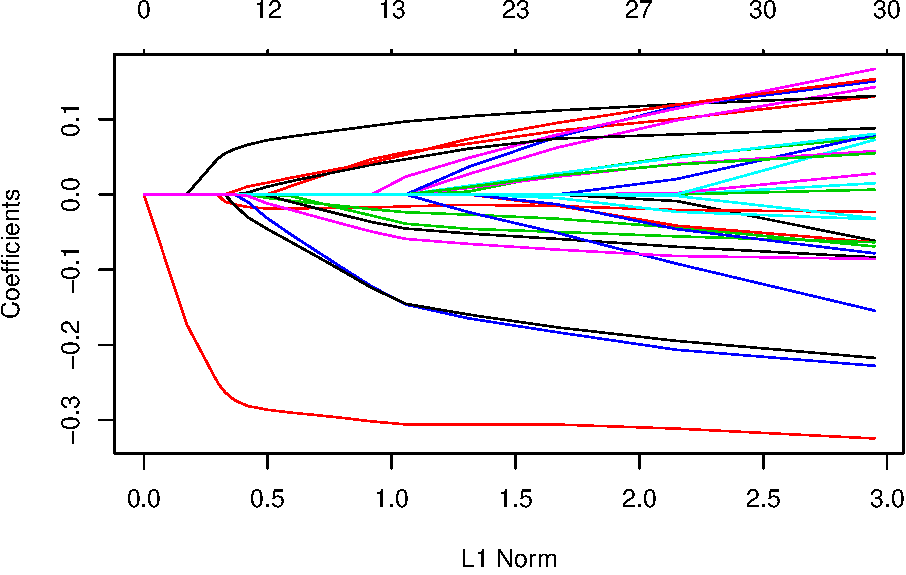
\includegraphics{Methods_comparison_files/figure-latex/unnamed-chunk-17-1.pdf}

\begin{Shaded}
\begin{Highlighting}[]
\KeywordTok{print}\NormalTok{(clrlasso)}
\end{Highlighting}
\end{Shaded}

\begin{verbatim}
## 
## Call:  glmnet(x = clrx, y = y, family = "binomial", alpha = 1, lambda = seq(0.015,      2, 0.01), standardize = FALSE) 
## 
##        Df      %Dev Lambda
##   [1,]  0 1.769e-15  1.995
##   [2,]  0 1.769e-15  1.985
##   [3,]  0 1.769e-15  1.975
##   [4,]  0 1.769e-15  1.965
##   [5,]  0 1.769e-15  1.955
##   [6,]  0 1.769e-15  1.945
##   [7,]  0 1.769e-15  1.935
##   [8,]  0 1.769e-15  1.925
##   [9,]  0 7.783e-15  1.915
##  [10,]  0 1.769e-15  1.905
##  [11,]  0 1.769e-15  1.895
##  [12,]  0 1.769e-15  1.885
##  [13,]  0 1.769e-15  1.875
##  [14,]  0 1.769e-15  1.865
##  [15,]  0 1.769e-15  1.855
##  [16,]  0 1.769e-15  1.845
##  [17,]  0 1.769e-15  1.835
##  [18,]  0 1.769e-15  1.825
##  [19,]  0 1.769e-15  1.815
##  [20,]  0 1.769e-15  1.805
##  [21,]  0 7.783e-15  1.795
##  [22,]  0 1.769e-15  1.785
##  [23,]  0 1.769e-15  1.775
##  [24,]  0 1.769e-15  1.765
##  [25,]  0 1.769e-15  1.755
##  [26,]  0 1.769e-15  1.745
##  [27,]  0 1.769e-15  1.735
##  [28,]  0 1.769e-15  1.725
##  [29,]  0 1.769e-15  1.715
##  [30,]  0 1.769e-15  1.705
##  [31,]  0 1.769e-15  1.695
##  [32,]  0 1.769e-15  1.685
##  [33,]  0 7.783e-15  1.675
##  [34,]  0 1.769e-15  1.665
##  [35,]  0 1.769e-15  1.655
##  [36,]  0 1.769e-15  1.645
##  [37,]  0 1.769e-15  1.635
##  [38,]  0 1.769e-15  1.625
##  [39,]  0 1.769e-15  1.615
##  [40,]  0 1.769e-15  1.605
##  [41,]  0 1.769e-15  1.595
##  [42,]  0 1.769e-15  1.585
##  [43,]  0 1.769e-15  1.575
##  [44,]  0 1.769e-15  1.565
##  [45,]  0 7.783e-15  1.555
##  [46,]  0 1.769e-15  1.545
##  [47,]  0 1.769e-15  1.535
##  [48,]  0 1.769e-15  1.525
##  [49,]  0 1.769e-15  1.515
##  [50,]  0 1.769e-15  1.505
##  [51,]  0 1.769e-15  1.495
##  [52,]  0 1.769e-15  1.485
##  [53,]  0 1.769e-15  1.475
##  [54,]  0 1.769e-15  1.465
##  [55,]  0 1.769e-15  1.455
##  [56,]  0 1.769e-15  1.445
##  [57,]  0 7.783e-15  1.435
##  [58,]  0 1.769e-15  1.425
##  [59,]  0 1.769e-15  1.415
##  [60,]  0 1.769e-15  1.405
##  [61,]  0 1.769e-15  1.395
##  [62,]  0 1.769e-15  1.385
##  [63,]  0 1.769e-15  1.375
##  [64,]  0 1.769e-15  1.365
##  [65,]  0 1.769e-15  1.355
##  [66,]  0 1.769e-15  1.345
##  [67,]  0 1.769e-15  1.335
##  [68,]  0 1.769e-15  1.325
##  [69,]  0 7.783e-15  1.315
##  [70,]  0 1.769e-15  1.305
##  [71,]  0 1.769e-15  1.295
##  [72,]  0 1.769e-15  1.285
##  [73,]  0 1.769e-15  1.275
##  [74,]  0 1.769e-15  1.265
##  [75,]  0 1.769e-15  1.255
##  [76,]  0 1.769e-15  1.245
##  [77,]  0 1.769e-15  1.235
##  [78,]  0 1.769e-15  1.225
##  [79,]  0 1.769e-15  1.215
##  [80,]  0 1.769e-15  1.205
##  [81,]  0 7.783e-15  1.195
##  [82,]  0 1.769e-15  1.185
##  [83,]  0 1.769e-15  1.175
##  [84,]  0 1.769e-15  1.165
##  [85,]  0 1.769e-15  1.155
##  [86,]  0 1.769e-15  1.145
##  [87,]  0 1.769e-15  1.135
##  [88,]  0 1.769e-15  1.125
##  [89,]  0 1.769e-15  1.115
##  [90,]  0 1.769e-15  1.105
##  [91,]  0 1.769e-15  1.095
##  [92,]  0 1.769e-15  1.085
##  [93,]  0 7.783e-15  1.075
##  [94,]  0 1.769e-15  1.065
##  [95,]  0 1.769e-15  1.055
##  [96,]  0 1.769e-15  1.045
##  [97,]  0 1.769e-15  1.035
##  [98,]  0 1.769e-15  1.025
##  [99,]  0 1.769e-15  1.015
## [100,]  0 1.769e-15  1.005
## [101,]  0 1.769e-15  0.995
## [102,]  0 1.769e-15  0.985
## [103,]  0 1.769e-15  0.975
## [104,]  0 1.769e-15  0.965
## [105,]  0 7.783e-15  0.955
## [106,]  0 1.769e-15  0.945
## [107,]  0 1.769e-15  0.935
## [108,]  0 1.769e-15  0.925
## [109,]  0 1.769e-15  0.915
## [110,]  0 1.769e-15  0.905
## [111,]  0 1.769e-15  0.895
## [112,]  0 1.769e-15  0.885
## [113,]  0 1.769e-15  0.875
## [114,]  0 1.769e-15  0.865
## [115,]  0 1.769e-15  0.855
## [116,]  0 1.769e-15  0.845
## [117,]  0 7.783e-15  0.835
## [118,]  0 1.769e-15  0.825
## [119,]  0 1.769e-15  0.815
## [120,]  0 1.769e-15  0.805
## [121,]  0 1.769e-15  0.795
## [122,]  0 1.769e-15  0.785
## [123,]  0 1.769e-15  0.775
## [124,]  0 1.769e-15  0.765
## [125,]  0 1.769e-15  0.755
## [126,]  0 1.769e-15  0.745
## [127,]  0 1.769e-15  0.735
## [128,]  0 1.769e-15  0.725
## [129,]  0 7.783e-15  0.715
## [130,]  0 1.769e-15  0.705
## [131,]  0 1.769e-15  0.695
## [132,]  0 1.769e-15  0.685
## [133,]  0 1.769e-15  0.675
## [134,]  0 1.769e-15  0.665
## [135,]  0 1.769e-15  0.655
## [136,]  0 1.769e-15  0.645
## [137,]  0 1.769e-15  0.635
## [138,]  0 1.769e-15  0.625
## [139,]  0 1.769e-15  0.615
## [140,]  0 1.769e-15  0.605
## [141,]  0 7.783e-15  0.595
## [142,]  0 1.769e-15  0.585
## [143,]  0 1.769e-15  0.575
## [144,]  0 1.769e-15  0.565
## [145,]  0 1.769e-15  0.555
## [146,]  0 1.769e-15  0.545
## [147,]  0 1.769e-15  0.535
## [148,]  0 1.769e-15  0.525
## [149,]  0 1.769e-15  0.515
## [150,]  0 1.769e-15  0.505
## [151,]  0 1.769e-15  0.495
## [152,]  0 1.769e-15  0.485
## [153,]  0 7.783e-15  0.475
## [154,]  0 1.769e-15  0.465
## [155,]  0 1.769e-15  0.455
## [156,]  0 1.769e-15  0.445
## [157,]  0 1.769e-15  0.435
## [158,]  0 1.769e-15  0.425
## [159,]  0 1.769e-15  0.415
## [160,]  0 1.769e-15  0.405
## [161,]  0 1.769e-15  0.395
## [162,]  0 1.769e-15  0.385
## [163,]  1 1.275e-03  0.375
## [164,]  1 7.497e-03  0.365
## [165,]  1 1.355e-02  0.355
## [166,]  1 1.944e-02  0.345
## [167,]  1 2.517e-02  0.335
## [168,]  1 3.074e-02  0.325
## [169,]  1 3.615e-02  0.315
## [170,]  1 4.141e-02  0.305
## [171,]  1 4.651e-02  0.295
## [172,]  1 5.146e-02  0.285
## [173,]  1 5.626e-02  0.275
## [174,]  1 6.091e-02  0.265
## [175,]  1 6.541e-02  0.255
## [176,]  1 6.976e-02  0.245
## [177,]  1 7.396e-02  0.235
## [178,]  1 7.802e-02  0.225
## [179,]  2 8.230e-02  0.215
## [180,]  2 8.806e-02  0.205
## [181,]  2 9.359e-02  0.195
## [182,]  2 9.891e-02  0.185
## [183,]  2 1.040e-01  0.175
## [184,]  2 1.089e-01  0.165
## [185,]  2 1.135e-01  0.155
## [186,]  3 1.181e-01  0.145
## [187,]  3 1.240e-01  0.135
## [188,]  5 1.319e-01  0.125
## [189,]  8 1.422e-01  0.115
## [190,] 10 1.557e-01  0.105
## [191,] 12 1.711e-01  0.095
## [192,] 12 1.860e-01  0.085
## [193,] 12 1.999e-01  0.075
## [194,] 12 2.125e-01  0.065
## [195,] 13 2.256e-01  0.055
## [196,] 20 2.457e-01  0.045
## [197,] 23 2.683e-01  0.035
## [198,] 27 2.910e-01  0.025
## [199,] 30 3.162e-01  0.015
\end{verbatim}

\begin{Shaded}
\begin{Highlighting}[]
\NormalTok{clrlasso_coef<-}\KeywordTok{coef}\NormalTok{(clrlasso,}\DataTypeTok{s=}\FloatTok{0.10}\NormalTok{)}
\KeywordTok{sum}\NormalTok{(}\KeywordTok{abs}\NormalTok{(clrlasso_coef)}\OperatorTok{>}\DecValTok{0}\NormalTok{)}
\end{Highlighting}
\end{Shaded}

\begin{verbatim}
## [1] 13
\end{verbatim}

\begin{Shaded}
\begin{Highlighting}[]
\NormalTok{selected_clrlasso<-}\KeywordTok{which}\NormalTok{(}\KeywordTok{as.numeric}\NormalTok{(}\KeywordTok{abs}\NormalTok{(}\KeywordTok{coef}\NormalTok{(clrlasso, }\DataTypeTok{s=}\FloatTok{0.1}\NormalTok{)))}\OperatorTok{>}\DecValTok{0}\NormalTok{)[}\OperatorTok{-}\DecValTok{1}\NormalTok{]; }
\end{Highlighting}
\end{Shaded}

The indices of selected variables (abs(coef)\textgreater{}0)

\begin{Shaded}
\begin{Highlighting}[]
\NormalTok{selected_clrlasso<-selected_clrlasso}\OperatorTok{-}\DecValTok{1}
\NormalTok{taxa_id<-}\KeywordTok{colnames}\NormalTok{(x_Crohn)[selected_clrlasso]}

\KeywordTok{write.csv}\NormalTok{(}\KeywordTok{data.frame}\NormalTok{(selected_clrlasso,taxa_id),}\StringTok{"./Generated_datasets/results_clrlasso_Crohn12.csv"}\NormalTok{)}
\end{Highlighting}
\end{Shaded}

\section{BEME day1 data}\label{beme-day1-data-2}

\chapter{Selbal: selection of balances}\label{selbal}

\section{Crohn disease data}\label{crohn-disease-data-3}

\begin{Shaded}
\begin{Highlighting}[]
\NormalTok{y<-y_Crohn  }
\end{Highlighting}
\end{Shaded}

For binary outcomes (logistic regression), selbal requires y to be
factor.

If y is numeric selbal implements linear regression.

\begin{Shaded}
\begin{Highlighting}[]
\NormalTok{x<-x_Crohn }
\KeywordTok{colnames}\NormalTok{(x)<-(}\DecValTok{1}\OperatorTok{:}\KeywordTok{ncol}\NormalTok{(x))}

\NormalTok{selbal_Crohn<-}\KeywordTok{selbal}\NormalTok{(}\DataTypeTok{x =}\NormalTok{ x, }\DataTypeTok{y =}\NormalTok{ y, }\DataTypeTok{logt=}\NormalTok{T, }\DataTypeTok{maxV=}\DecValTok{12}\NormalTok{)}
\end{Highlighting}
\end{Shaded}

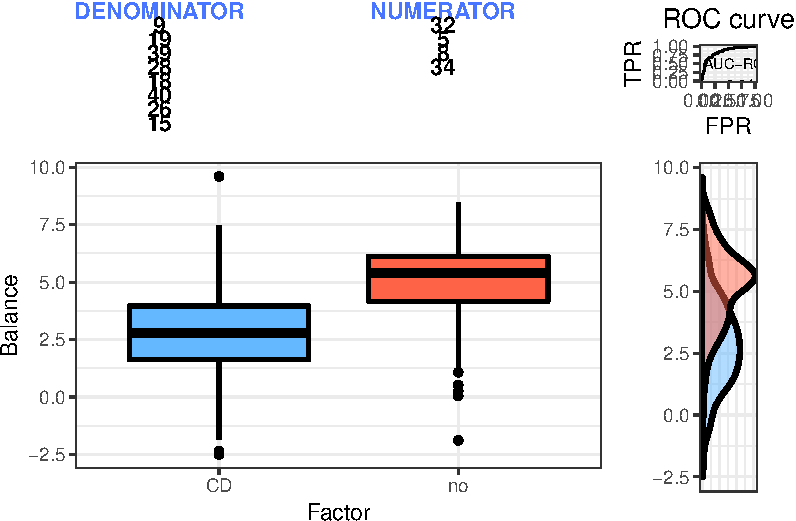
\includegraphics{Methods_comparison_files/figure-latex/unnamed-chunk-20-1.pdf}

\begin{Shaded}
\begin{Highlighting}[]
\NormalTok{selected_selbal<-}\KeywordTok{as.numeric}\NormalTok{(}\KeywordTok{c}\NormalTok{(selbal_Crohn[[}\DecValTok{6}\NormalTok{]][,}\DecValTok{1}\NormalTok{],selbal_Crohn[[}\DecValTok{6}\NormalTok{]][,}\DecValTok{2}\NormalTok{]))}
\end{Highlighting}
\end{Shaded}

\begin{verbatim}
## Warning: NAs introduced by coercion
\end{verbatim}

\begin{Shaded}
\begin{Highlighting}[]
\NormalTok{id.na<-}\KeywordTok{which}\NormalTok{(}\KeywordTok{is.na}\NormalTok{(selected_selbal))}
\NormalTok{selected_selbal<-selected_selbal[}\OperatorTok{-}\NormalTok{id.na]}
\NormalTok{selected_selbal<-}\KeywordTok{as.character}\NormalTok{(selected_selbal)}

\NormalTok{columns_selected_selbal<-}\KeywordTok{which}\NormalTok{(}\KeywordTok{colnames}\NormalTok{(x)}\OperatorTok\StringTok{ }\NormalTok{selected_selbal)}
\NormalTok{taxa_id<-}\KeywordTok{colnames}\NormalTok{(x_Crohn)[columns_selected_selbal]}

\KeywordTok{write.csv}\NormalTok{(}\KeywordTok{data.frame}\NormalTok{(columns_selected_selbal, taxa_id),}\StringTok{"./Generated_datasets/results_selbal_Crohn12.csv"}\NormalTok{)}
\end{Highlighting}
\end{Shaded}

\section{BEME day1 data}\label{beme-day1-data-3}

\chapter{Concordance of variables selected by the three
methods}\label{comparison}

\section{Crohn disease data}\label{crohn-disease-data-4}

\begin{Shaded}
\begin{Highlighting}[]
\NormalTok{d_selbal<-}\KeywordTok{read.csv}\NormalTok{(}\StringTok{"./Generated_datasets/results_selbal_Crohn12.csv"}\NormalTok{, }\DataTypeTok{header =}\NormalTok{ T)}
\NormalTok{d_clrlasso<-}\KeywordTok{read.csv}\NormalTok{(}\StringTok{"./Generated_datasets/results_clrlasso_Crohn12.csv"}\NormalTok{, }\DataTypeTok{header =}\NormalTok{ T)}
\NormalTok{d_codalasso<-}\KeywordTok{read.csv}\NormalTok{(}\StringTok{"./Generated_datasets/results_codalasso_Crohn12.csv"}\NormalTok{, }\DataTypeTok{header =}\NormalTok{ T)}

\CommentTok{#(d_selbal[,2], d_clrlasso[,2], d_codalasso[,2])}
  
\NormalTok{taxa_selected<-}\KeywordTok{list}\NormalTok{(d_clrlasso[,}\DecValTok{2}\NormalTok{], d_codalasso[,}\DecValTok{2}\NormalTok{], d_selbal[,}\DecValTok{2}\NormalTok{])}
\NormalTok{taxa.id_selected<-}\KeywordTok{list}\NormalTok{(d_clrlasso[,}\DecValTok{3}\NormalTok{], d_codalasso[,}\DecValTok{3}\NormalTok{], d_selbal[,}\DecValTok{3}\NormalTok{])}


\NormalTok{venn.plot <-}\StringTok{ }\KeywordTok{venn.diagram}\NormalTok{(taxa_selected , }\OtherTok{NULL}\NormalTok{, }\DataTypeTok{fill=}\KeywordTok{c}\NormalTok{(}\StringTok{"magenta"}\NormalTok{, }\StringTok{"blue"}\NormalTok{, }\StringTok{"lightblue"}\NormalTok{), }
                          \DataTypeTok{alpha=}\KeywordTok{c}\NormalTok{(}\FloatTok{0.5}\NormalTok{,}\FloatTok{0.5}\NormalTok{,}\FloatTok{0.5}\NormalTok{), }\DataTypeTok{cex =} \DecValTok{2}\NormalTok{, }\DataTypeTok{cat.fontface=}\DecValTok{4}\NormalTok{, }
                          \DataTypeTok{category.names=}\KeywordTok{c}\NormalTok{(}\StringTok{"clr+lasso"}\NormalTok{, }\StringTok{"coda-lasso"}\NormalTok{, }\StringTok{"selbal"}\NormalTok{),}
                          \DataTypeTok{main=}\StringTok{"Concordance of selected taxa for Crohn data"}\NormalTok{)}
\KeywordTok{grid.draw}\NormalTok{(venn.plot)}
\end{Highlighting}
\end{Shaded}

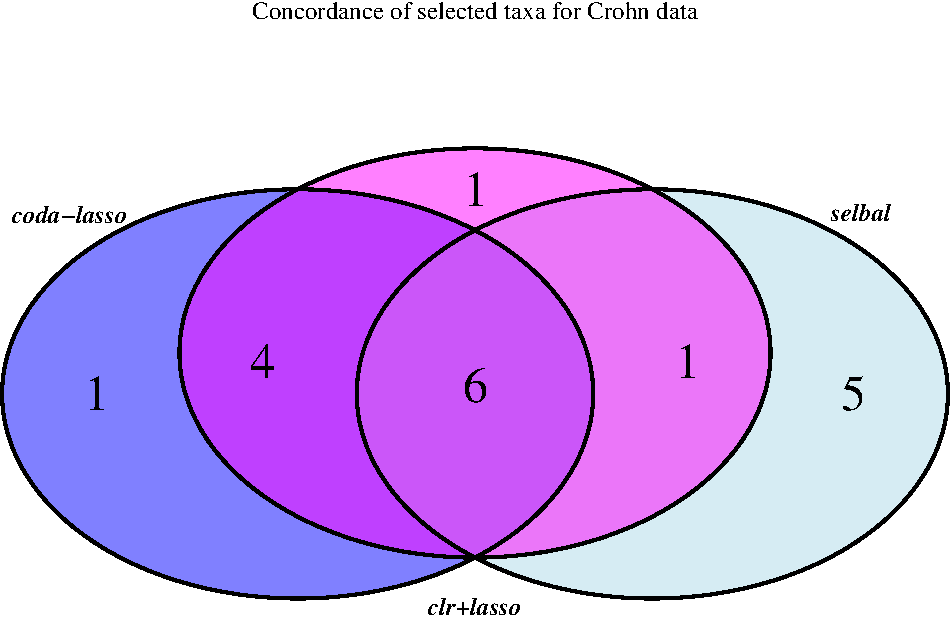
\includegraphics{Methods_comparison_files/figure-latex/unnamed-chunk-21-1.pdf}

\begin{Shaded}
\begin{Highlighting}[]
\NormalTok{taxa.id <-}\StringTok{ }\KeywordTok{venn}\NormalTok{(taxa.id_selected, }\DataTypeTok{show.plot=}\OtherTok{FALSE}\NormalTok{)}
\NormalTok{taxa <-}\StringTok{ }\KeywordTok{venn}\NormalTok{(taxa_selected, }\DataTypeTok{show.plot=}\OtherTok{FALSE}\NormalTok{)}

\NormalTok{inters_taxa.id <-}\StringTok{ }\KeywordTok{attr}\NormalTok{(taxa.id,}\StringTok{"intersections"}\NormalTok{)}
\NormalTok{inters_taxa <-}\StringTok{ }\KeywordTok{attr}\NormalTok{(taxa,}\StringTok{"intersections"}\NormalTok{)}

\KeywordTok{lapply}\NormalTok{(inters_taxa, head) }
\end{Highlighting}
\end{Shaded}

\begin{verbatim}
## $A
## [1] "10"
## 
## $B
## [1] "27"
## 
## $C
## [1] "15" "18" "26" "28" "34"
## 
## $`A:B`
## [1] "2"  "31" "33" "48"
## 
## $`A:C`
## [1] "8"
## 
## $`A:B:C`
## [1] "5"  "9"  "19" "32" "39" "40"
\end{verbatim}

\begin{Shaded}
\begin{Highlighting}[]
\KeywordTok{lapply}\NormalTok{(inters_taxa.id, head) }
\end{Highlighting}
\end{Shaded}

\begin{verbatim}
## $A
## [1] "g__Faecalibacterium"
## 
## $B
## [1] "o__Lactobacillales_g__"
## 
## $C
## [1] "g__Blautia"           "g__Dorea"             "g__Oscillospira"     
## [4] "g__Adlercreutzia"     "o__Clostridiales_g__"
## 
## $`A:B`
## [1] "g__Parabacteroides" "g__Prevotella"      "g__Lachnospira"    
## [4] "g__Bilophila"      
## 
## $`A:C`
## [1] "g__Bacteroides"
## 
## $`A:B:C`
## [1] "f__Peptostreptococcaceae_g__" "g__Eggerthella"              
## [3] "g__Dialister"                 "g__Roseburia"                
## [5] "g__Streptococcus"             "g__Aggregatibacter"
\end{verbatim}

\section{BEME day1 data}\label{beme-day1-data-4}

\bibliography{book.bib}


\end{document}
